
%------------------------------------------------------------------------
\section{Evaluation}
\TODO

%-------------------------------------------------------------------------
\subsection{Procedural Models}
\label{sec:sampling}

In order to analyze how reconstruction algorithms perform w.r.t. varying sampling density, we describe a simple sampling algorithm ~\cite{ohrhallinger2016hnn} which creates an approximate $\epsilon$-sampling on cubic B{\'e}zier curves.

First we sample the segments of the B{\'e}zier curve densely along its parametrization.
Then we determine the normal $n_i$ at each curve sample $s_i \in S$ as orthogonal to the edge connecting its neighbor samples on the curve.
The largest empty disc at $s_i$ can be established by $s_i, n_i$ and querying each other curve sample $s_j \in \{S \setminus s_i\}$ by setting the disc center $c_j=s_i+tn_i,\|cs_i\|=\|cs_j\|$, which we solve and then add the $c_j$ having the largest radius of all empty discs to the set of medial axis points $M$.
After having sampled the medial axis, we can simply estimate the lfs for each $s_i$ by locating its nearest neighbor in $M$ and its distance.
Note that this computation is not exact due to discretizing the original curve as well as floating point precision, however computing medial axis thus lfs exactly is a hard and expensive task~\cite{aichholzer09medialaxis},~\cite{attali09medialaxis}, and since $\epsilon$-sampling requires an upper bound on distance, but the curve is also discretized, the chosen samples should be mostly within that bound.
In order to sample the curve with a given $\epsilon$, we now start with any curve sample $s_i$ (or any on its boundary if the curve is open) and iterate over successive samples along the curve while $\|s_i,s_j\|/\mbox{lfs}<\epsilon$ and choose the last valid one as next point in our $\epsilon$-sampling.

Since we have computed the lfs, we can further perturb samples in its terms to simulate feature size varying noise.
We retain the sampling density by just moving each sample along their normal which was incidentally determined by the fitting of the empty discs.

%-------------------------------------------------------------------------
\subsection{Procedural Textures}


~\cite{mehra2010visibility}: \url{http://www.cs.unc.edu/~ravishm/robustPointVisibility_smi_10_files/data/DATA_version_2.zip}
~\cite{lee2000curve}: data sets bottle and fish (with SO)


%-------------------------------------------------------------------------
\subsection{Evaluation Criteria}

Amplitude Distribution\\


Periodograms\\

Power spectrum estimate\\



%-------------------------------------------------------------------------
\subsection{Comparative Study}




%-------------------------------------------------------------------------
\subsection{Results}


\begin{figure}
	\centering
	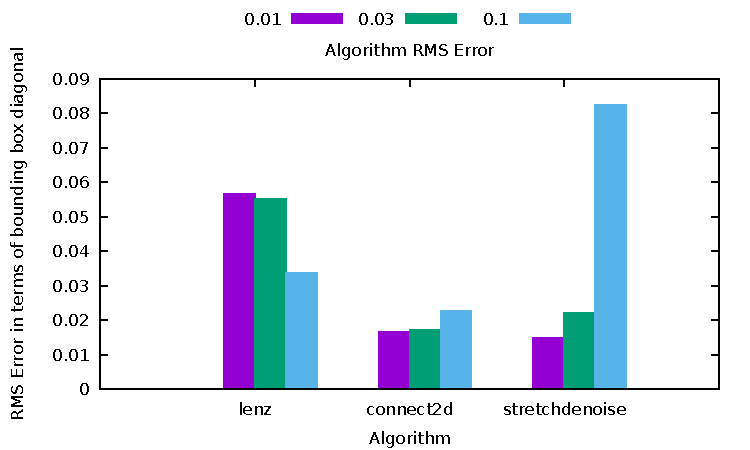
\includegraphics[width=3in]{fig/noisy.pdf}
	\caption{RMS Error of reconstructed curves from ground truth for the point sets used in Figure~\ref{fig:eval-exact}, with the points perturbed with noise of $\delta=0.01, 0.03$ and $0.1$. ({\em run-noisy.sh})}
	\label{fig:eval-noisy}
\end{figure}

\begin{figure}
	\centering
	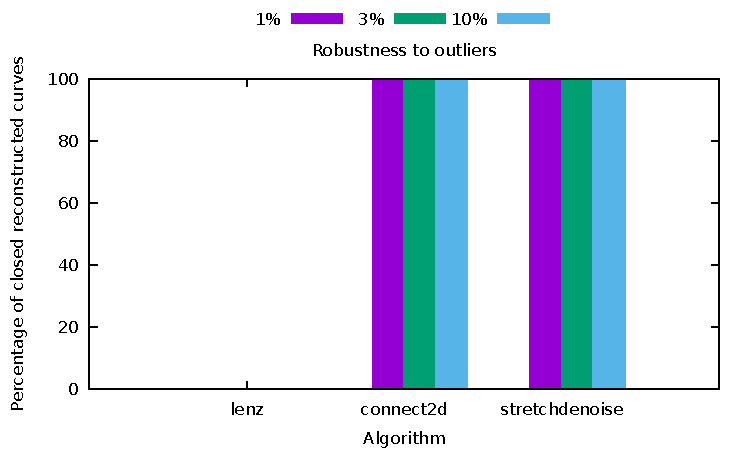
\includegraphics[width=3in]{fig/outliers.pdf}
	\caption{Percentage of closed reconstructed curves for the point sets used in Figure~\ref{fig:eval-exact}, with a share of $1\%, 3\%$ and $10\%$ outliers added. ({\em run-outliers.sh})}
	\label{fig:eval-outliers}
\end{figure}






%------------------------------------------------------------------------- 